% !TEX root = ../../../thesis.tex
The fabrication followed the method outlined in Section \ref{sec:method-sample-fabrication}. Due to a machine malfunction we deposited \qty{113}{\nano\meter} of \ce{Nb} instead of of \qty{90}{\nano\meter}\footnote{This was measured using an Atomic Force Microscope (AFM) by M. Westerdijk.}. The fine structures we made using the Focussed Ion Beam (FIB), can be seen in Figure \ref{fig:CP1.2H-SEM-images}.

\begin{figure}
	\begin{subfigure}[b]{0.3\textwidth}
		\centering
		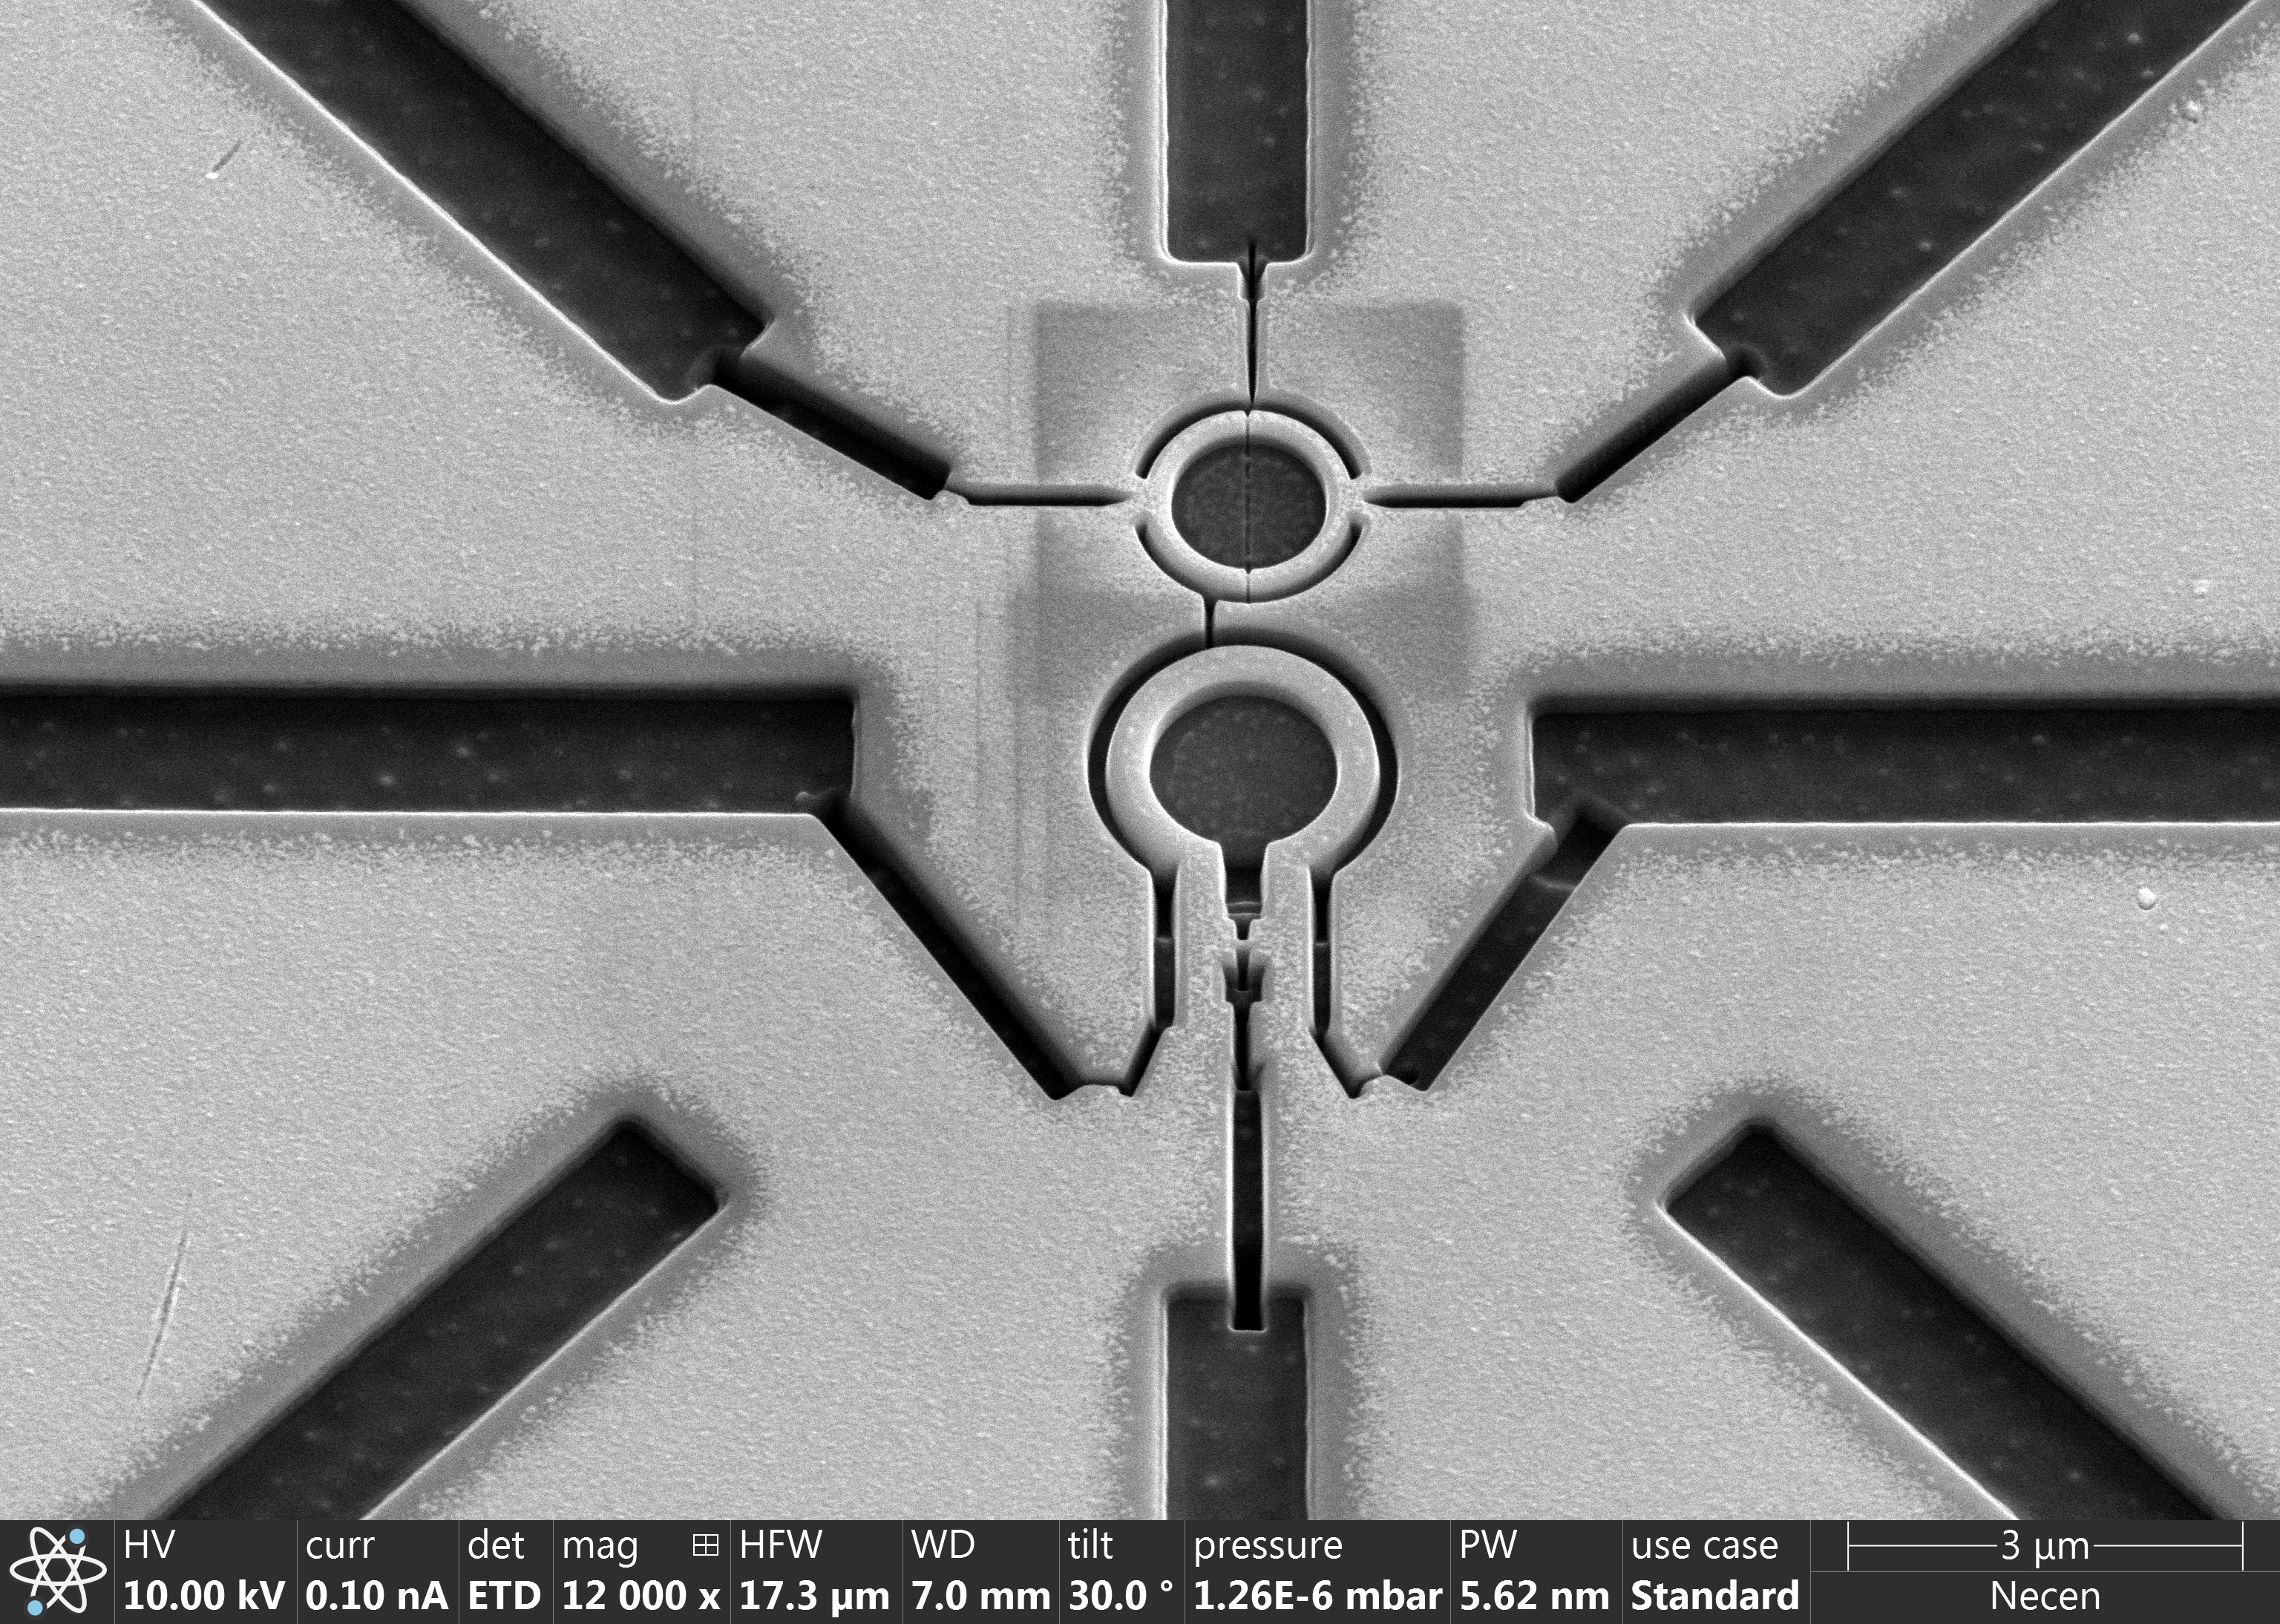
\includegraphics[width=\textwidth]{figures/samples/CP1/CP1.2H_SEM_overview.jpg}
		\subcaption{Overview of the fine structures. The thick leads go to \qty{300}{\micro\meter} by \qty{300}{\micro\meter} contact pads. On top we see the dc-SQUID and on the bottom the junction loop.}
	\end{subfigure}
	\hfill
	\begin{subfigure}[b]{0.3\textwidth}
		\centering
		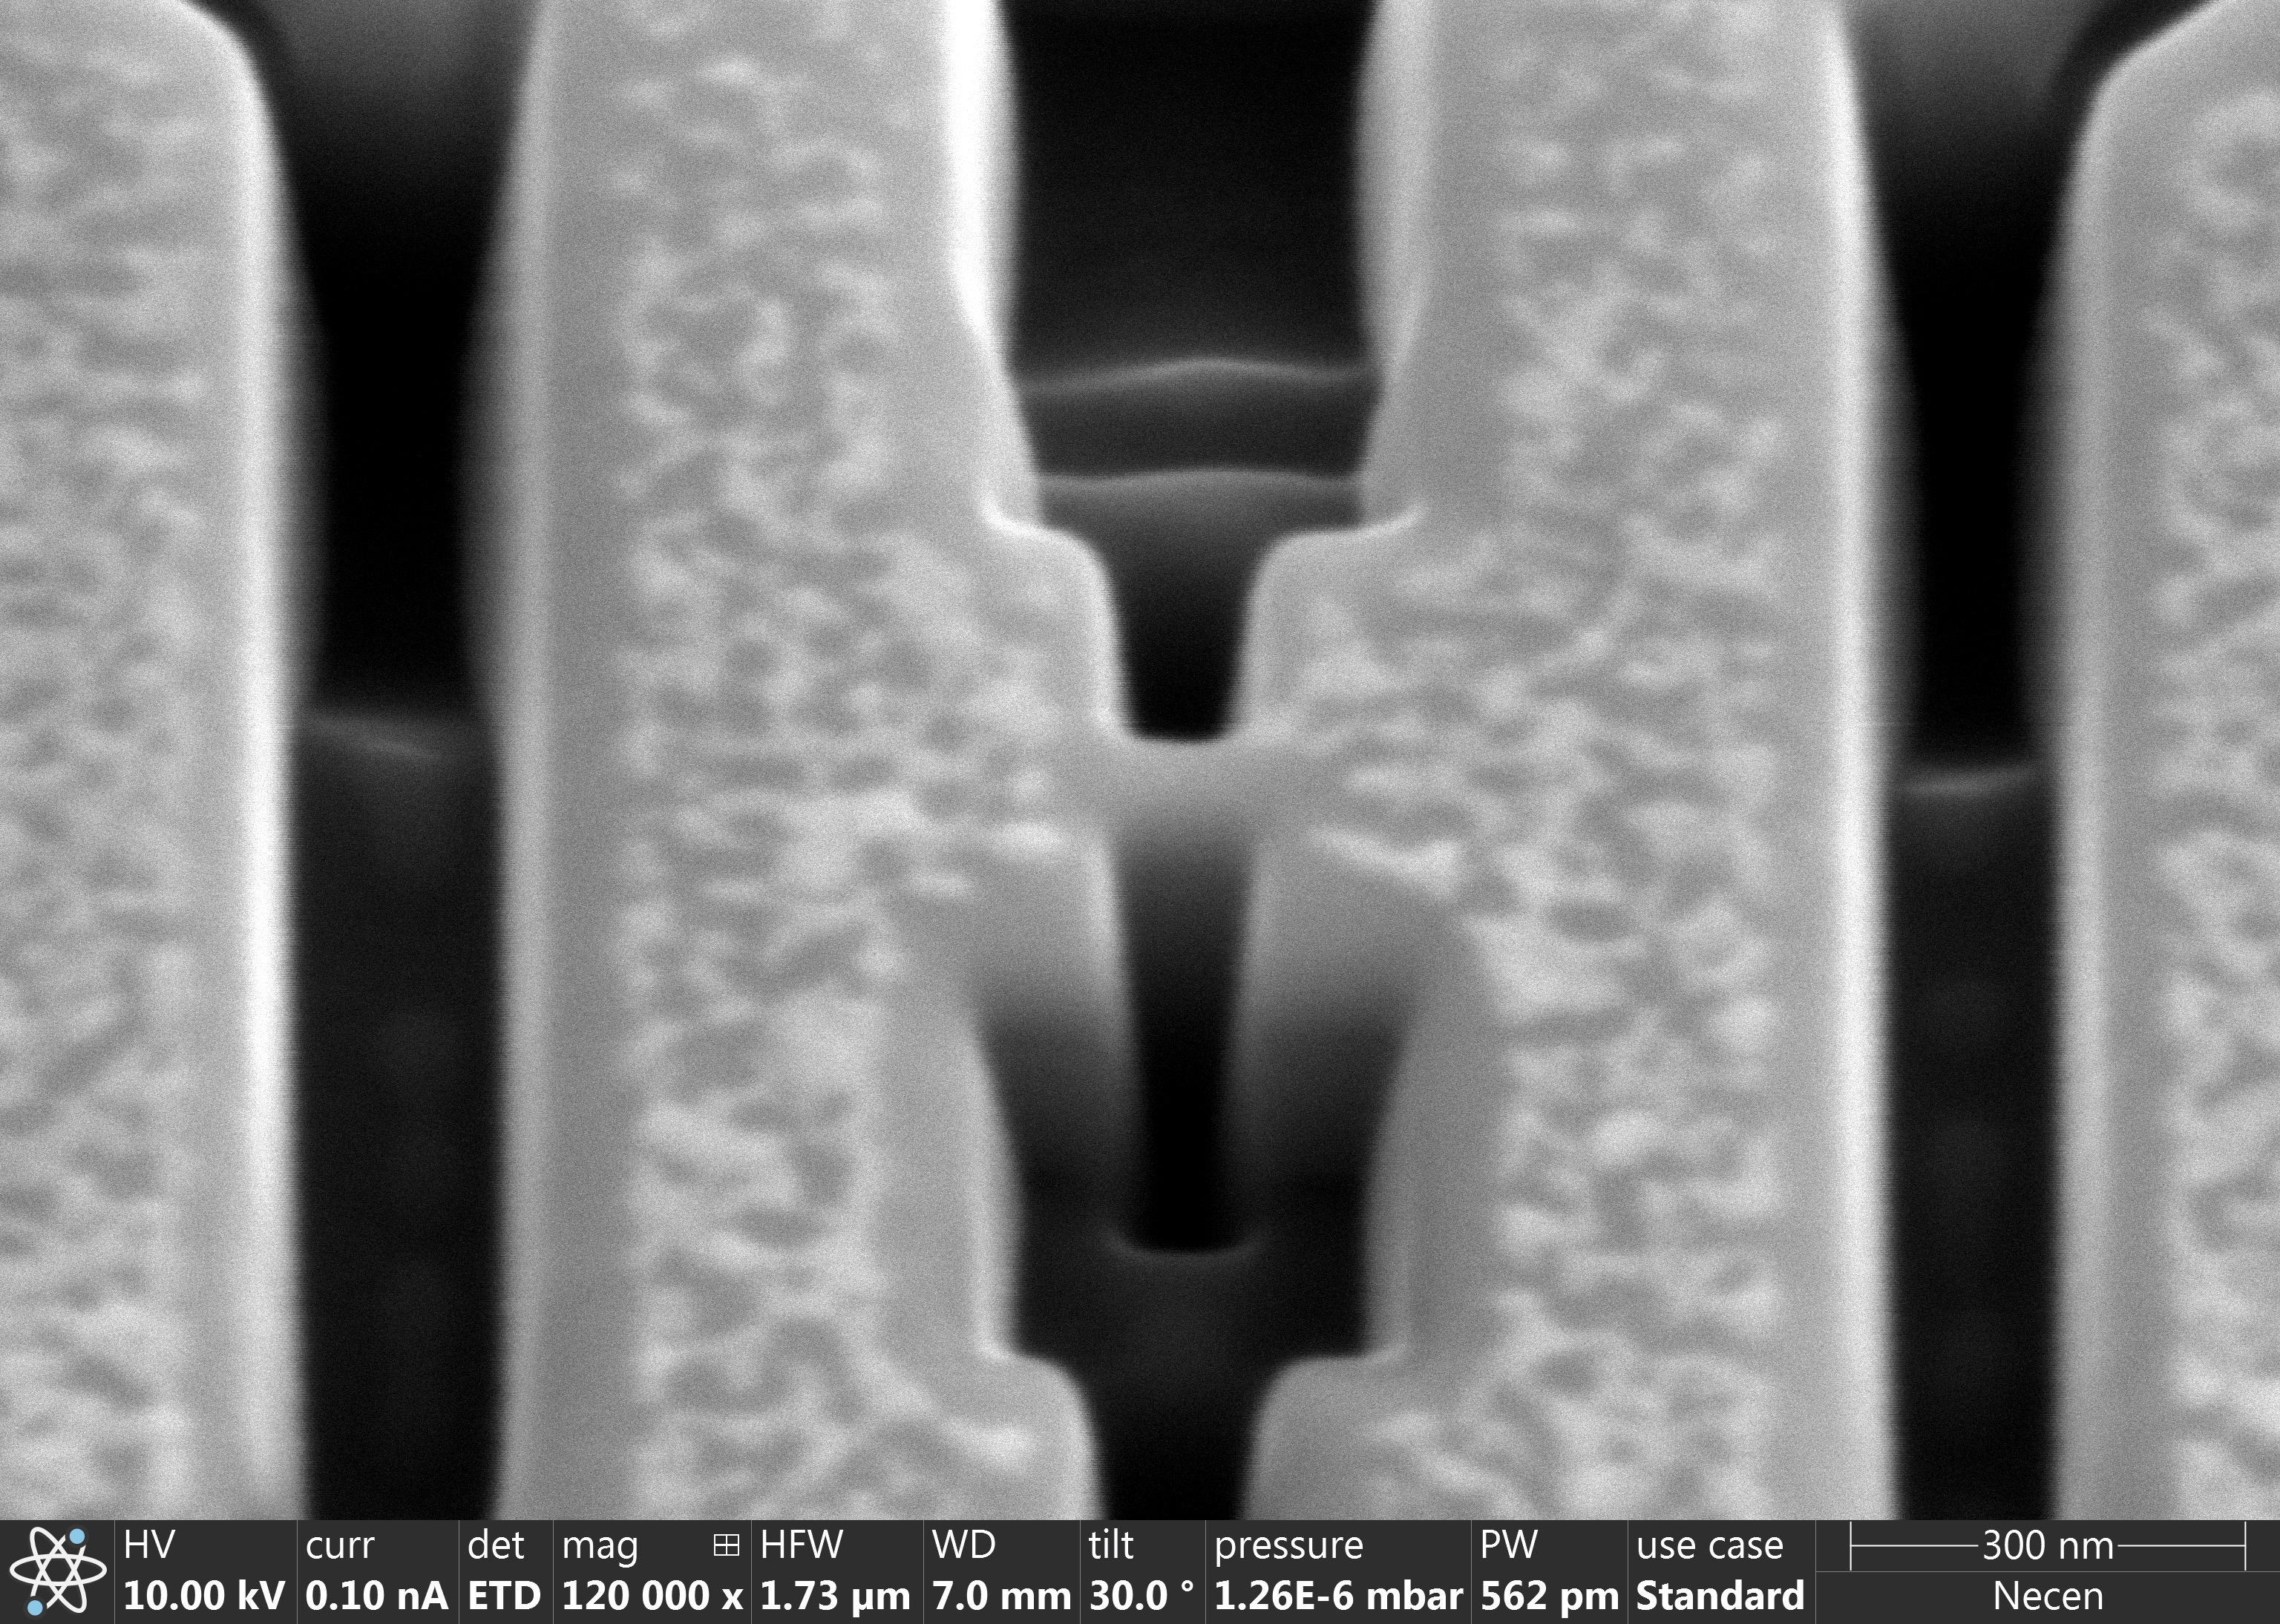
\includegraphics[width=\textwidth]{figures/samples/CP1/CP1.2H_SEM_junction.jpg}
		\subcaption{Zoomed in view of the junction, the size of the junction is \qty{100}{\nano\meter} by \qty{80}{\nano\meter}.}
	\end{subfigure}
	\hfill
	\begin{subfigure}[b]{0.3\textwidth}
		\centering
		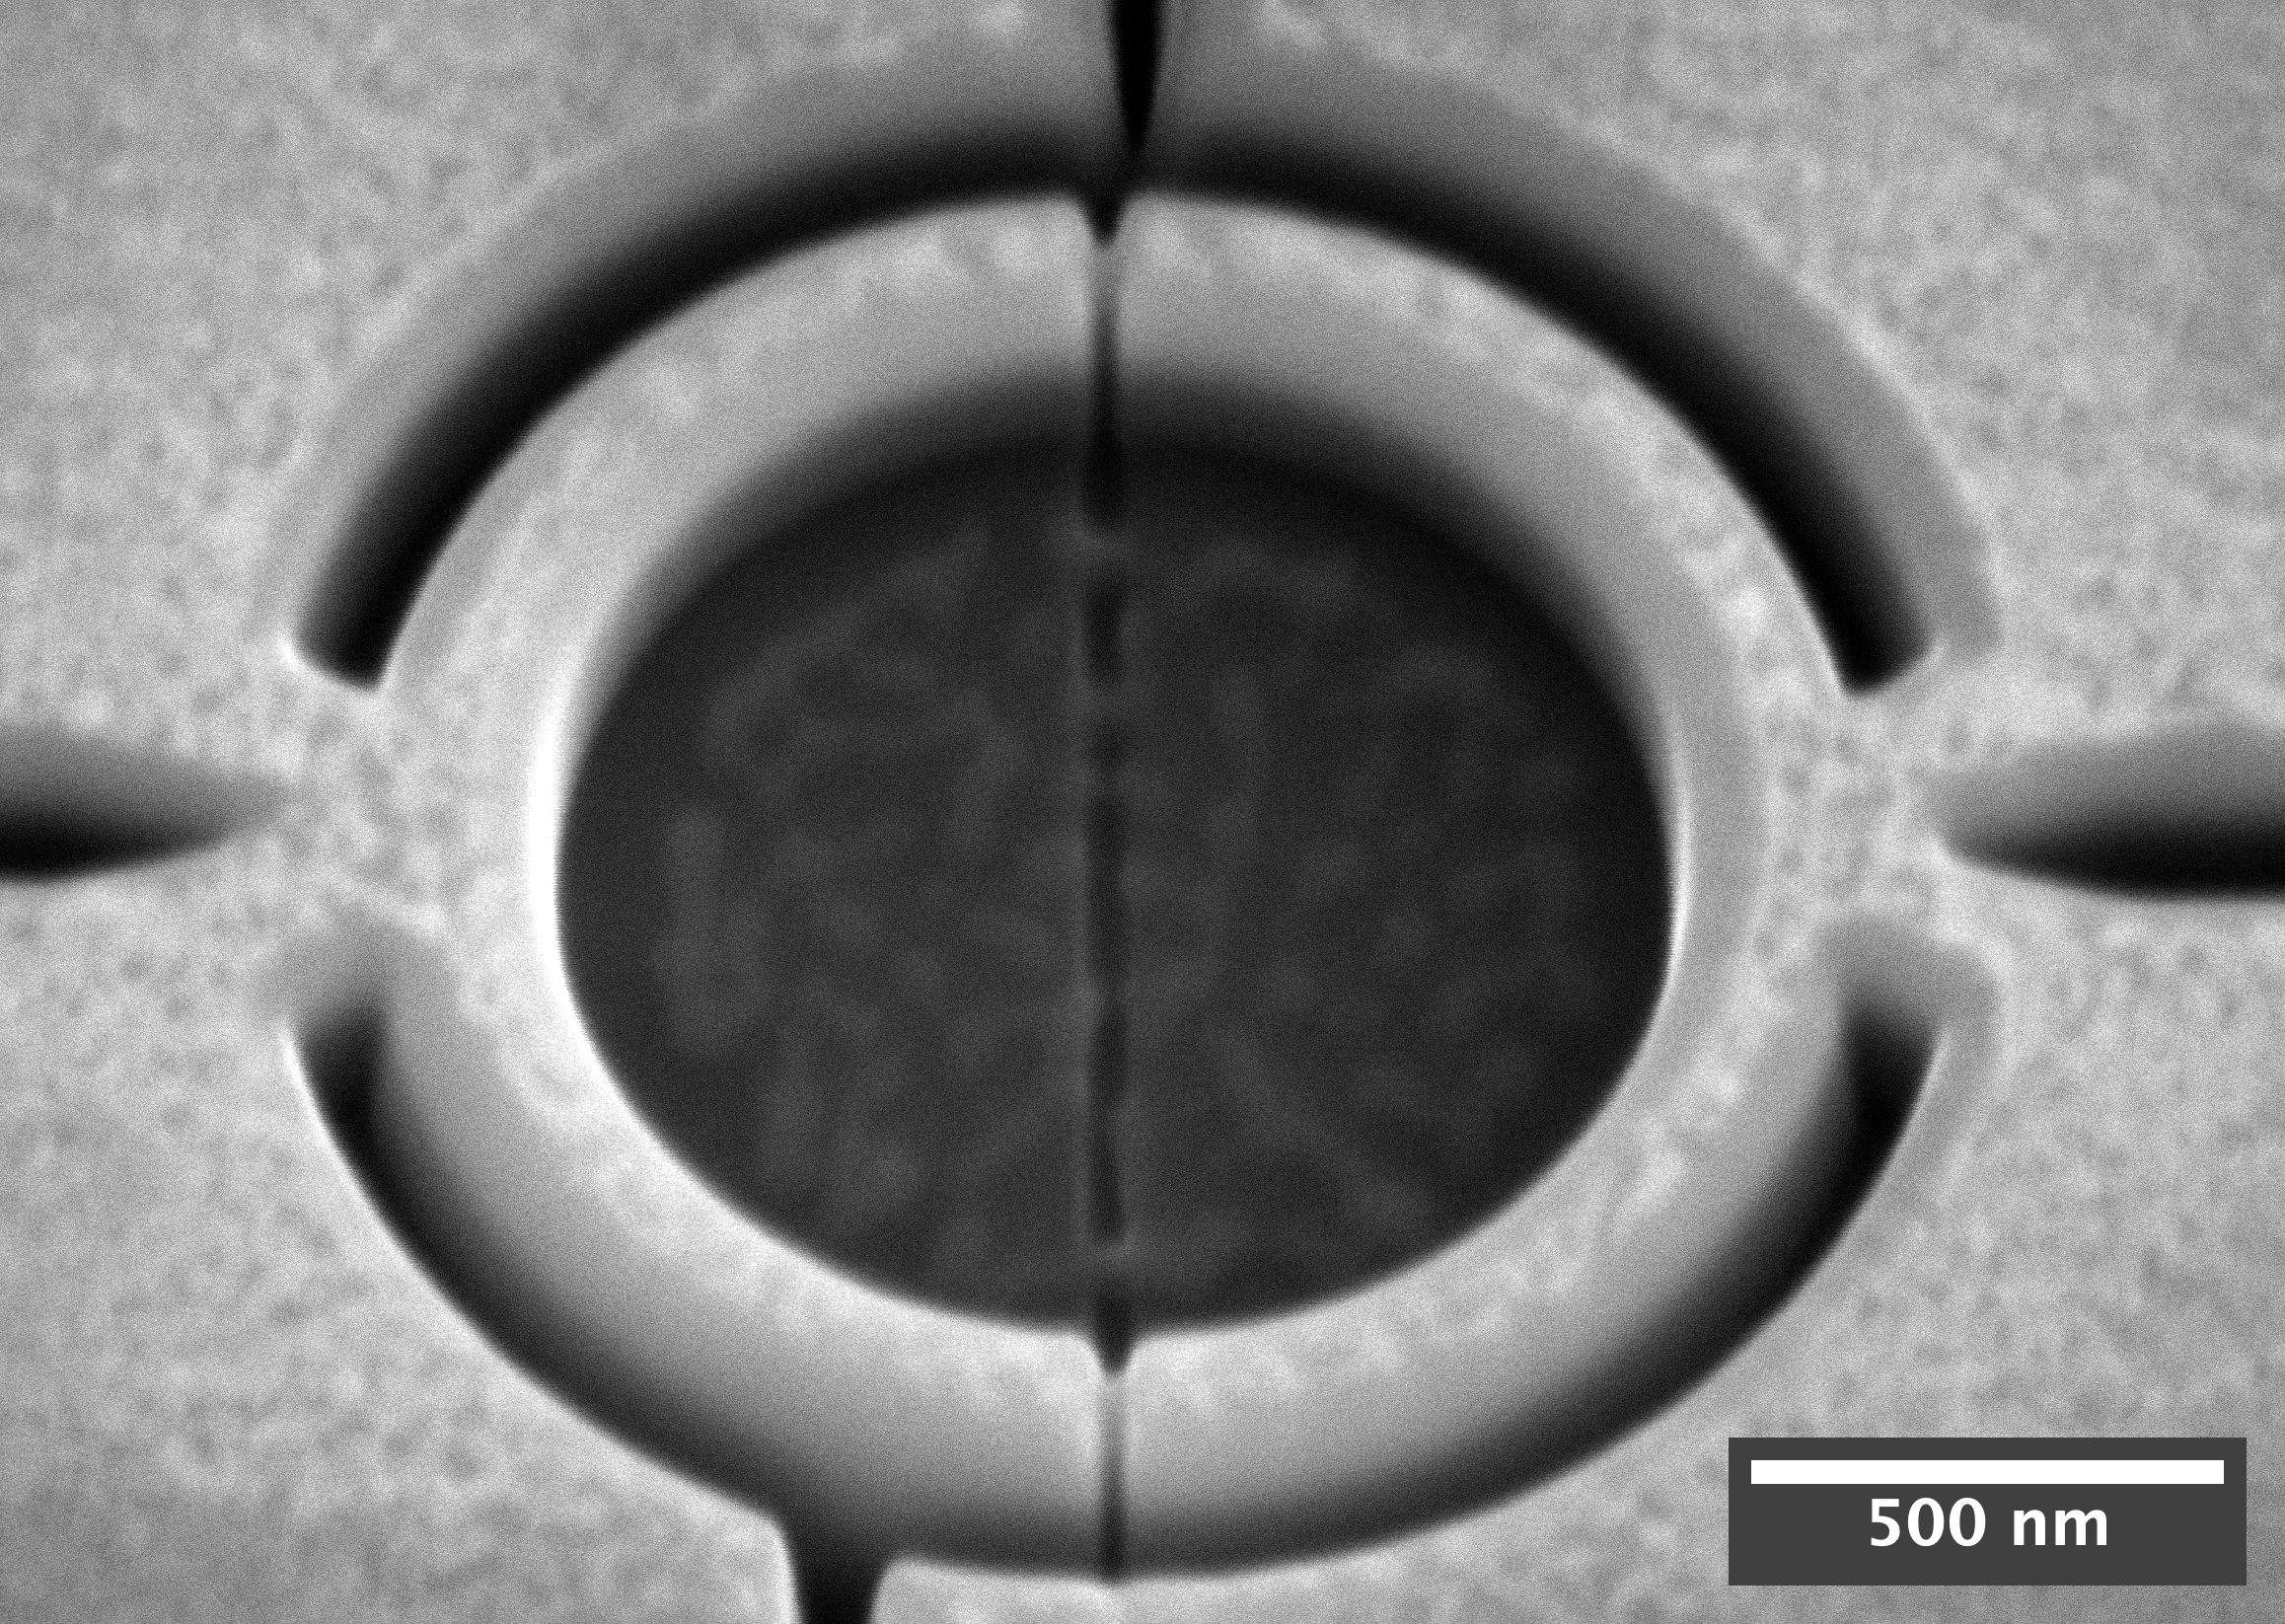
\includegraphics[width=\textwidth]{figures/samples/CP1/CP1.2H_SEM_SQUID.jpg}
		\subcaption{Zoomed in view of the dc-SQUID. The inner and outer diameters are \qty{1.195}{\micro\meter} and \qty{1.608}{\micro\meter} respectively. The length of the junction is \qty{19}{\nano\meter}.}
	\end{subfigure}

	\caption{Fine structures of sample CP1.2H after the FIB.}
	\label{fig:CP1.2H-SEM-images}
\end{figure}